\chapter{Apprentissage Automatique}

\section{Introduction}
L'apprentissage automatique, en anglais est l'appelé "machine Learning" .
Représente une discipline passionnante au cœur de l'intelligence artificielle. 
Ce domaine cherche à développer des modèles informatiques capables d'apprendre à partir de l'expérience et d'améliorer leurs performances au fil du temps, sans être explicitement programmés.
 

\section{L'apprentissage Automatique }
L’apprentissage automatique est un type d'intelligence artificielle (IA), c’est une science qui permet aux ordinateurs d'apprendre sans être explicitement programmés « Arthur Samuel, 1959 ». Plus précisément, l'apprentissage automatique fait référence au développement, l'analyse et l'implémentation de méthodes qui permettent à une machine (au sens large) d'évoluer et de remplir des tâches associées à une intelligence artificielle grâce à un processus d'apprentissage. Cet apprentissage permet d'avoir un système qui s'optimise en fonction de l'environnement, les expériences et les résultats observés.
Dans le domaine médicale, l’apprentissage automatique a été conçu pour réaliser l'analyse de données médicales, surtout lorsque l'évolution numérique a fourni des moyens (capteurs) peu coûteux permettant de recueillir et de stocker des informations importantes liées aux patients et maladies. Par exemple, les algorithmes d'apprentissage sont utiles au médecin lors du diagnostic des patients, afin d'améliorer la vitesse, la précision et la fiabilité de son diagnostic.

\section{Types d’Apprentissage Automatique }
Il existe fondamentalement quatre types d’apprentissage automatique : Supervisé, semi-supervisé et non-supervisé et Apprentissage par renforcement. 
Dans notre étude, nous utilisons l’apprentissage supervisé pour construire des modèles pour la prédiction des maladies.
Dans la suite de cette section, nous allons présenter les deux types d’apprentissage les plus utilisés qui sont l’apprentissage supervisé et apprentissage non supervisé.

\begin{figure}[h]
\centering
\includegraphics[scale=0.8]{Images/Chapiter2/Types d’Apprentissage Automatique.PNG}
\caption{Les différentes méthodes d'apprentissage automatique.}
\label{fig:01}
\end{figure}

\subsection{Apprentissage Supervisé }
Dans l'apprentissage supervisé, l'ordinateur est fourni avec des exemples d'entrées qui sont étiquetés avec les sorties souhaitées. Le but de cette méthode est que l'algorithme puisse « apprendre » en comparant sa sortie réelle avec les sorties « apprises » pour trouver des erreurs et modifier le modèle en conséquence. 
L'objectif des algorithmes d'apprentissage supervisé est d'apprendre une fonction qui mappe les vecteurs de caractéristiques (entrées) aux étiquettes (sortie), sur la base d'exemples de paires entrée-sortie.  

Comme il est illustré dans la Figure 1 l’apprentissage supervisé peut être utilisé pour deux types de tâches principales : la classification et la régression. 
Les algorithmes de classification cherchent à prédire la classe ou la catégorie à laquelle appartient une donnée d'entrée tandis que les algorithmes de régression servent à prédire une valeur numérique continue à partir de variables d'entrée. Dans ce travail, nous nous intéressons aux méthodes de classification.
\subsection{Apprentissage Non-Supervisé  }
Dans l'apprentissage non supervisé, les données sont non étiquetées, de sorte que l'algorithme d'apprentissage trouve tout seul des points communs parmi ses données d'entrée. Les données non étiquetées étant plus abondantes que les données étiquetées, les méthodes d'apprentissage automatique qui facilitent l'apprentissage non supervisé sont particulièrement utiles.
L'objectif de l'apprentissage non supervisé peut être aussi simple que de découvrir des modèles cachés dans un ensemble de données.
Les plus fréquents problèmes connus dans ce type sont :
\begin{itemize}
\item Le clustering qui consiste à regrouper un ensemble d’éléments hétérogènes sous forme de sous-groupes homogènes.

\item La réduction de dimension qui consiste à prendre des données dans un espace de grande dimension, et à les remplacer par des données dans un espace de plus petite dimension sans perdre la variance .
\end{itemize}


\section{Définition de classification }
Un modèle de classification est un modèle d'apprentissage automatique qui attribue des étiquettes ou des catégories à des instances d'entrée en les associant à un ensemble fini de classes prédéfinies. 
L'objectif est de créer une fonction qui peut généraliser à de nouvelles données et assigner correctement des classes à des observations inconnues en fonction des modèles appris à partir des données d'entraînement. 
Les classes peuvent être binaires (deux classes, comme oui/non) ou multinomiales (plus de deux classes), et le modèle cherche à discriminer entre ces classes en fonction des caractéristiques des données d'entrée.

\section{Les types de classification }
Dans cette partie, nous présentons les types de classification :
\newpage
\subsection{La classification binaire (Binary classification) }
La classification binaire (ou la classification binomiale) est une transformation de données qui vise à répartir les membres d'un ensemble dans deux groupes disjoints selon que l'élément possède ou non une propriété / fonctionnalité donnée, mais peut également être interprété comme vrai et faux, 1 et 0, ou toute autre combinaison de deux valeurs. 
Par exemple : tests médicaux visant à déterminer si un patient est atteint d'une certaine maladie ou non. 

\begin{figure}[!h]
\centering
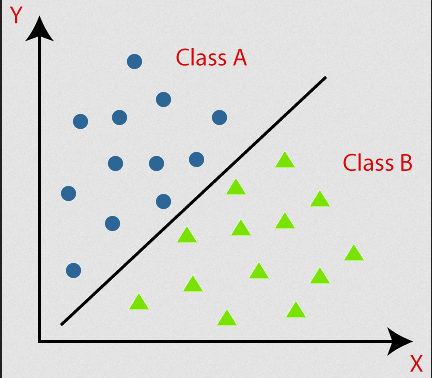
\includegraphics[scale=0.5]{Images/Chapiter2/La classification binaire.png}
\caption{Exemple de problème de classification binaire.}
\label{fig:02}
\end{figure}

\begin{itemize}
\item L’image montre qu’il y a deux classes : classe A et classe B.
\end{itemize}
\begin{center}
\end{center}


\subsection{La classification multi-classe }
La classification multi-classe désigne une tâche de classification comportant plus de deux classes, par exemple, La classification des visages, classification des espèces végétales...Ect.
 Un jeu de données multi-classe n’a qu’une seule classe en sortie, comme dans la classification binaire.
 \newpage

\subsection{La classification multi-lable }
Jusqu'à présent, chaque instance était toujours affectée à une seule classe. Dans certains cas, le classificateur peut produire plusieurs classes pour chaque instance.
   Par exemple, un classificateur pour reconnaître des types de maladies : que faire s'il reconnaît plusieurs symptômes en même temps ? Bien entendu, il doit noter chaque symptôme associé à une maladie spécifique. Supposons qu'un classificateur ait été formé pour reconnaître trois symptômes : « fatigue, nausée et température élevée ».
Ainsi, lorsqu’il apparaît « fatigué et une forte température ».
Il devrait produire [1, 0, 1] (c'est-à-dire : fatigué oui, nausée non, fièvre oui.) Un système de classification qui produit plusieurs binaires est appelé système de classification multi-étiquettes.

\begin{figure}[!h]
\centering
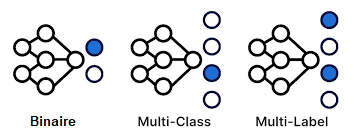
\includegraphics[scale=1]{Images/Chapiter2/La classification multi-lable.png}
\caption{Exemple de problème de classification binaire , multi-classe et multi-lable .}
\label{fig:03}
\end{figure}

\section{Techniques de Classification }
Dans cette partie, nous présentons les algorithmes de classification :

\subsection{Les k plus proches voisins (KNN) }
L’algorithme des k plus proches voisins en anglais est l'appelé « K-Nearest Neighbors (KNN) » est un algorithme de classification supervisé. Chaque observation de l’ensemble d’apprentissage est représentée par un point dans un espace à n dimensions ou n est le nombre de variables prédictives. Pour prédire la classe d’une observation, on cherche les k points les plus proches de cet exemple. La classe de la variable cible, est celle qui est la plus représentée parmi les k plus proches voisins. Il existe des variantes de l’algorithme ou on pondère les k observations en fonction de leur distance à l’exemple dont on veut classer les observations les plus éloignées de notre exemple seront considérées comme moins importantes.

\begin{figure}[!h]
\centering
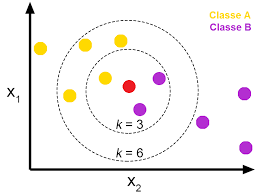
\includegraphics[scale=0.8]{Images/Chapiter2/Les k plus proches voisins (KNN).png}
\caption{Pour k = 3 la classe majoritaire du point central est la classe B, mais si on change la valeur du voisinage k = 6 la classe majoritaire devient la classe A .}
\label{fig:03}
\end{figure}

\subsection{k-means }
L’algorithme des k-moyennes en anglais est l'appelé « k-means » est un algorithme non supervisé. Chaque observation est représentée par un point dans un espace à n dimensions ou n est le nombre de variables descriptives.
À partir d’un ensemble d’apprentissage de $M$ observations $[X^{1}, \ldots, X^{M}]$ cet algorithme va repartir ces observations en k clusters de manière à ce que la distance euclidienne qui sépare les points au centre de gravité du groupe auquel ils sont affectés soit minimale. Les étapes de l’algorithme sont :

\begin{itemize}
\item Choisir k points qui représentent la position moyenne des clusters.
\item répéter jusqu’à stabilisation des points centraux :
\begin{itemize}
\item[-] affecter chacun des M points au plus proche des k points centraux.
\item[-]mettre à jour les points centraux en calculant les centres de gravité des k cluster.
\end{itemize}
\end{itemize}

\begin{figure}[!h]
\centering
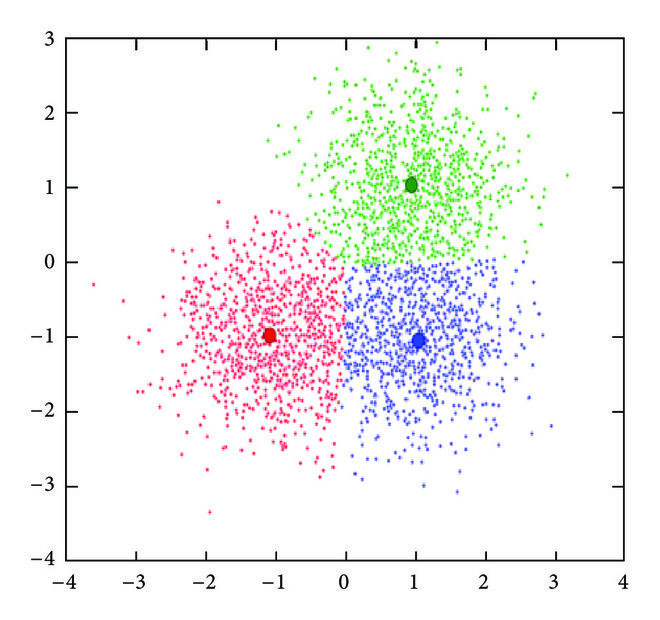
\includegraphics[width=8cm, height=6cm]{Images/Chapiter2/k-means.png}
\caption{L’algorithme k-means regroupe les données en k cluster, ici k = 3. Les centres de gravité sont représentés par de petit cercle.}
\label{fig:04}
\end{figure}

\subsection{Régression Logistique}
L'analyse de régression est souvent utilisée pour faire des prédictions, comprendre les variables indépendantes par rapport à la variable dépendante et étudier la forme de leur relation.
Dans des circonstances limitées, l'analyse de régression peut être utilisée pour déduire la relation causale entre la variable indépendante et la variable dépendante.
La régression est un algorithme robuste lorsqu'il s'agit de classer des ensembles de problèmes, et a une fonction logistique (fonction sigmoïde) au cœur de celui-ci. Dans cet algorithme, les valeurs d'entrée sont combinées en fonction de coefficients ou de poids pour donner les valeurs de sortie/prédites. 

\begin{figure}[!h]
\centering
\includegraphics[scale=1]{Images/Chapiter2/Régression Logistique .png}
\caption{Modèle la régression logistique.}
\label{fig:05}
\end{figure}
\newpage
\subsection{Machine à Vecteurs de Supports (S V M) }
Machine à Vecteurs de Supports en anglais cela l'appelé « Support Vector Machine » est l’un des algorithmes d’apprentissage supervisé les plus populaires, utilisé pour les problèmes de classification et de régression. 
Cependant, il est principalement utilisé pour les problèmes de classification dans l’apprentissage automatique. Le but de l’algorithme SVM est de créer la meilleure ligne ou limite de décision qui peut séparer l’espace à n dimensions en classes afin que nous puissions facilement mettre le nouveau point de données dans la bonne classe à l’avenir.

\begin{figure}[!h]
\centering
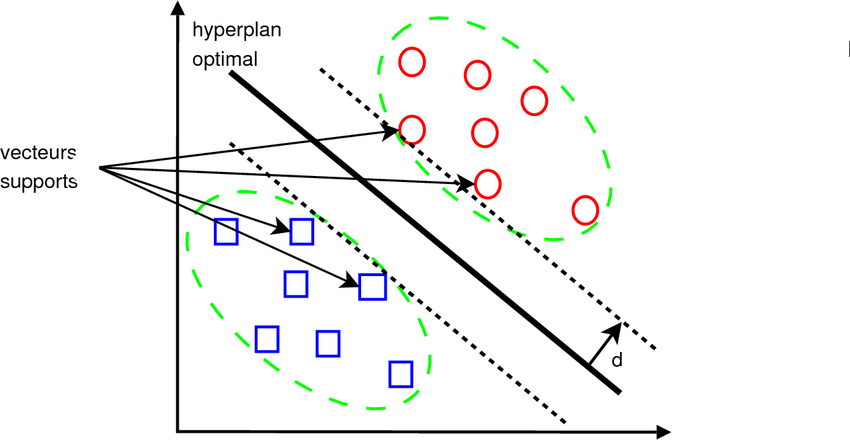
\includegraphics[scale=0.5]{Images/Les-vecteurs-de-support.png}
\caption{Un diagramme d'un hyperplan avec des vecteurs de support dans un espace vectoriel à deux dimensions.}
\label{fig:06}
\end{figure}


\begin{itemize}
\item[-] La figure \ref{fig:06} montre un exemple simple d'un hyperplan avec des vecteurs de support. Cette technique peut être utilisée pour séparer deux classes de points dans un espace vectoriel, ce qui est utile pour des tâches d'apprentissage automatique telles que la classification et la régression.
L'objectif d'un hyperplan avec des vecteurs de support est de trouver la meilleure séparation possible entre deux classes de points dans un espace vectoriel. Cela peut être utilisé pour des tâches de classification, telles que la reconnaissance d'image ou le traitement du langage naturel.
\end{itemize}

\subsection{Apprentissage profondeur }
Apprentissage profond en anglais est l'appelé « Deep Learning » est un type d'intelligence artificielle dérivé du machine Learning (apprentissage automatique) où la machine est capable d'apprendre par elle-même, contrairement à la programmation où elle se contente d'exécuter à la lettre des règles prédéterminées.

\begin{figure}[h]
\centering
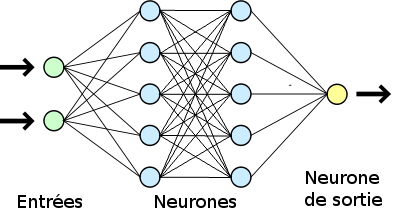
\includegraphics[scale=0.8]{Images/Chapiter2/Apprentissage profondeur.png}
\caption{Architecture Apprentissage profondeur.}
\label{fig:07}
\end{figure}

La figure \ref*{fig:07} fournie montre une architecture d'apprentissage profond composée de plusieurs couches empilées les unes sur les autres. Chaque couche est composée d'un certain nombre de neurones artificiels qui sont interconnectés. 
Les neurones sont responsables de traiter les informations et de les transmettre à la couche suivante.

\begin{itemize}
\item \textbf{Couches d'entrée} : Elles reçoivent les données brutes, comme des images ou du texte.
\item \textbf{Couches cachées} : Elles traitent les données et extraient des caractéristiques de plus en plus complexes.
\item \textbf{Couche de sortie} : Elle produit la sortie finale, comme une classification ou une prédiction.
\end{itemize}

\newpage
\section{Comparaison entre techniques de classification}

\label{tab:01}
\begin{table}[h]

\begin{tabular}{| m{3cm}| m{6cm}| m{6cm}|}
\hline
 \textbf{Techniques de Classification} & \textbf{Avantages} & \textbf{Inconvénients} \\ 
 \hline
 \textbf{KNN} & - Simple à concevoir &
 \begin{itemize}
 \item[-]Sensible aux bruits.
 \item[-]Pour un nombre de variable prédictives très grands, le calcul de la distance devient très coûteux.
 \end{itemize}
 
 \\  
 \hline
\textbf{ k-means} & -implémentable pour des grands volumes de données & 
 \begin{itemize}
 \item[-]Le choix du paramètre k n’est pas découvert mais choisi par l’utilisateur .
 \item[-] La solution dépend des k centre de gravité choisi lors de l’initialisation
 \end{itemize}
 \\
 \hline
 \textbf{Régression Logistique} & - Ses résultats sont faciles à interpréter. & 
 \begin{itemize}
\item[-] La phase d’apprentissage peut être longue car l’optimisation des coefficients est complexe. 
\item[-]Sa linéarité empêche la prise en compte des interactions entre les variables.
\end{itemize}
 \\
 \hline
 \textbf{S V M} &
 \begin{itemize} 
 \item[-]Il permet de traiter des problèmes de classification non linéaire complexe.
 \item[-]Les SVM constituent une alternative aux réseaux de neurones car plus faciles à entraîner.
 \end{itemize}
 & 
 \begin{itemize} 
 \item[-] Les SVM peuvent être lents à entraîner sur de grands ensembles de données.
 \item[-] Cela peut affecter la précision du modèle et le rendre moins fiable.
 \end{itemize}
 \\
 \hline
 \textbf{Apprentissage profondeur} &
 \begin{itemize}
  \item[-] Adaptabilité à Divers Domaines.
  \item[-] Performances Exceptionnelles dans des Tâches Complexes.
  
  \end{itemize}
 & 
 \begin{itemize}
 \item[-]Interprétabilité Limitée.
 \item[-]Besoin d'Expertise Technique Élevée.
 
 \end{itemize}
\\
 \hline
\end{tabular}
\end{table}

\newpage
\section{Conclusion}
Dans ce chapitre, nous avons présenté les algorithmes d'apprentissage supervisé. 
Après avoir présenté les deux principaux types d’apprentissage automatique, une description détaillée de chaque méthode de classification a été fournie, en expliquant le principe de fonctionnement de chaque méthode ainsi que ses avantages et inconvénients.
Le chapitre suivant présente les méthodes d’apprentissage profondeur qui ont été appliquées dans le domaine de la santé.
